\documentclass{article}
\usepackage{blindtext}
\usepackage[utf8]{inputenc}
\usepackage[margin=1in]{geometry}
\usepackage{graphicx}
\usepackage{longtable}
\usepackage[backend=bibtex,style=numeric,citestyle=numeric]{biblatex}
\linespread{2}
\graphicspath{ {images/} }
\addbibresource{DissertationPart2.bib}
\title{An Exploration into Building Three Clients for JominiEngine\\ Deliverable One\\BSc Computer Systems}
\author{Rory Malcolm\\Heriot Watt School of Maths and Computer Science\\H00157560\\Supervisor: Hans-Wolfgang Loid\\Second Reader: Chris Fensch}
\date{\today}
\begin{document}

	\maketitle
	\newpage
	\tableofcontents
	\newpage
	\section{Introduction}
	\subsection{Aims}
	\subsubsection{Abstract}
	At Heriot Watt a historically accurate massively multiplayer online role playing game called “JominiEngine” has been created and improved over the years. JominiEngine aims to provide a serious game for prospective students to learn about the time period it is set from gameplay. It implements a client-server model, the client communicates with the server using Google's Protobuf communication layer.\\

	In this dissertation we aim to produce a number of JominiEngine clients for different platforms; a text based command line client, a client for Linux desktop and a mobile client on the Android operating system. The implementation of these clients aims to expand the accessibility of the JominiEngine, currently the client available for the game is used mostly for testing purposes. After their completion we will carry out usability studies, compare and contrast the user’s experiences with the features and complexities of each environment and how the development experience plays a role in the final product. The report will focus on the portability of the protocol implementation and if the current client server environment lends itself well to the expansion of JominiEngine onto new platforms.
	\subsubsection{Aims}
	Through the development of the three clients for the JominiEngine we aim to expand the accessibility of the game beyond the current implementation, which for the most part consists of the server and a demonstration client by giving users working, usable clients on multiple platforms. From the implementation of the mobile client we will learn more about how the JominiEngine gameplay can be transposed onto mobile phones, within the constraints that come packaged with the platform, and what effect this transposition has on the overall user opinion of the product. The desktop and text clients will provide me with a perception into what effect a robust user interface has on the user's experience of the product, comparing the simple text command line interface results from the usability study to that of the full graphic user interface will provide insight to this. We will also be able to infer the technical capability of clients for the JominiEngine; Massively Multiplayer Online Role Playing Games by definition must be able to accomodate for large amounts of connections at once and these clients, especially the text client, will allow for the development of an automated testing suite to ensure that the server is capable at this level or performance. Technical metrics that are harvested from unit tests and telemetry performed while these are running will tell the technical side of the story, comparisons can be made between the clients and what effect they have on the system they are currently running on, these will be used to make informed criticisms of the final implementation of the clients with regards to code quality and scalability.
	\subsection{Objectives}
	\begin{itemize}
	\item Produce three clients
	\item All of the clients should implement the current JominiEngine protocol as standard.
	\item One of the clients runs on a mobile operating system which operates over mobile internet.
	\item One of the clients runs on a standard linux operating system (eg. Ubuntu).
	\item One of the clients is a text based client for internal and testing use.
	\item Usability studies are conducted which show that the clients have been adapted to provide the best user experience for each platform’s constraints.
	\item The clients provide a scalable solution; multiple clients can run on a single computer with ease in order to test the constraints of the game server.
	\item The clients automatically find servers which are running on their local network and connect to them over the protocol. 
	\item As features are added to the server and protocol by other students working on JominiEngine my implementation of the clients should be flexible enough to easily incorporate any changes.
	\item Implement a client side caching system to reduce the load on the central server, increasing scalability.
	\item The user should be able to move their account between devices and clients.
\end{itemize}
	\subsection{Evaluation}
	The evaluation stage is the mechanism through which we establish wether the project has been successful and if so, to what degree. We can go through every objective and consider our experiences in implementing it, and what effect this had on the rest of the development process. The evaluation stage of this project will encompass a technical evaluation from which measurements about the performance of the clients will be extracted and compared and a user evaulation which will use a usability study to measure the opinion of users towards the clients and compare and contrast the scores between platforms.
	\section{Background}
	\subsection{Literature Review}
	The purpose of the literature review is to explore the academic literature that surrounds the topics that our project will be covering, to understand where current research lies and what the best practises in each of these fields are.
	\subsubsection{Game Design Decisions}
	As gaming moves beyond being a special interest hobby and into the mainstream the popularity of MMORPG’s has swelled; for example Blizzard Inc, the creator of the 2004 released World Of Warcraft reported in 2015, 11 years after the games release, that they had a player population of 5.6 million active users. Efforts to explore the popularity of MMORPGs have been carried out\cite{Christou:2012:EPP:2367616.2367630}, studies show that the usability of the game has a positive effect on engaging players but the popularity of the MMORPG genre cannot be inferred from this, only that well-made, usable games are attractive to players. There have been other attempts to analyse the community aspects of MMORPG’s effect on the player base\cite{DoThoseWhoPlay}, research has concluded that while players initially struggle to immerse themselves fully in the world after some effort is spent they find themselves inside of complex social systems which mimic and alter real life, some respondents reported that the social aspect was the most important part of their gaming experience. This aspect of gaming can only be found in multiplayer games where interaction with other players is possible. The study reflects on the fact that the World of Warcraft players it surveyed do not see a point in playing alone, the social aspect of the game is so great that they do not see their gaming experience as complete without it. This is explored further when looking at the\cite{Hainey:2011:DMO:2304793.2305216} difference between the way multiplayer gamers and single player gamers in higher education view their experiences, they noted that online gamers see competition, challenge and recognition to be much more important than offline gamers and that online gamers believed gaming to be “more of a social activity, less of a waste of time, more interesting, more worthwhile, more enjoyable, more valuable, more exciting and less of a lonely activity”. This yet again confirms the perception that online gaming and offline gaming, while in the same field of interest have separate mechanics and are different experiences gameplay wise and socially. We then can look at the personalisation aspect of MMORPG’s and how that effects the user’s perception of their gaming experience. Players feel RPGs place them in the context of the situations the game is providing and do not feel the character is a separate entity\cite{bowman:2012:EPP:2367616.2367630} this further strengthens the “MMORPGs are inherently social and personalised via a product of game mechanics" hypothesis. JominiEngine aims to become a serious game, these differ from normal games due to the context in which they are used. While normal games aim to pass the time, providing the player with entertainment, serious games aim to provide the player with a learning experience, a new method of studying. JominiEngine's historical accuracy aims to help a student of history familiarise themselves with the time period it is set and by playing they learn more about the context and actors at play during this period. This has been explored academically in the past\cite{seriousgames} and history especially has an avenue for study via serious games due to the fact they can immerse the user fully into the time and world of study.
	\subsubsection{Game Interface Decisions}
	When considering the implementation decisions for an MMORPG client it is important to understand how the user will be interfacing with the game and what options are best for the platform the user will be running the game on, taking into account the limitations and constraints of that platform. Most of the work surrounding mobile gaming interfaces explores the new experiences that can had due to the player have access to new sensors such as a accelerometer or the phone's GPRS service. However if we look at the mobile client we have to ask what are the limitations that are placed upon it via the hardware. Phones have smaller screens than desktop computers so there may need to be some modification of the user interface in order to account for this. As we have mentioned before, usability is a main driving factor in user attachment to games\cite{Christou:2012:EPP:2367616.2367630}, it is not enough for the client to offer a command line version for mobile and still have users come away from it as immersed; these interfaces are designed for machines which have hardware keyboards as their main method of communication. The mobile client's interface must be designed from the ground up for the platform, taking into account for example, the large touch screen most smartphones have. The user could navigate fiefs by dragging their fingers around a map similar to the current hexmap used in the test client implemented in Helen Rankin's masters thesis\cite{helenrankin}, this would provide a mobile-first user interface using techniques more natural to frequent users of the platform. The text client will use a Read, Evaluate, Print, Loop style interface that is common in command line applications such as Python's IDLE\cite{python}, the user is prompted input information by the program, the user then inputs the step they wish to take, the program evaluates their input, prints the output and the process is repeated again. Using such a common interface for command line tools alongside a help menu should make for a better and more familiar user experience.
	\subsubsection{Mobile Game Development}
	When considering development on a mobile platform we must first consider the mobile operating system that we wish to develop our app for; there are a lot of options available on the market but the two main players in the industry are iOS and Android. If we first look at iOS some problems arise that could hinder the development process, first of all to get access to the full suite of development tooling there is a subscription fee to publish apps and the XCode IDE which is used to develop  apps for iOS only runs on the Mac platform. There is tooling which aims to open up the development experience for iOS such as Microsoft's Xamarin\cite{Xamarin} which allows for a developer to write C\# code which cross compiles for running on both Android and iOS but this still requires a development license and an accessbile Mac machine for compiling the code to an executable which can run on an iPhone. Android on the other hand is fully open source and can be developed for on any platform, natively it runs Java code but there are a large number of languages which have been ported to the platform for running on its ART virtual machine such as Scala or Jython - an implementation of the Python programming language which compiles to Android RunTime bytecode.
	\subsubsection{Mobile Networking and its Effect on the Gaming Experience}
	There has been some research into the effects of mobile network’s temperamentally on a players gaming experience. One research paper\cite{6098224} looked at the frequency of disconnections on a wireless ad-hoc Quake3 server and found that the quality of connection meant that “the number of disconnections due to packet losses were so frequent that very few parties ended with all participating players “. Network stress’s effects on the MMORPG gaming experience has also been explored; Everquest2 was used as a testbed to monitor the effects of latency on a players “skill”, defined as the time it took for the time it took for players to complete tests in the game\cite{Fritsch:2005:ELN:1103599.1103623}. They found that at 1250ms of ping it became unplayable, however it is important to note that the context of this test was in a real time game and not a turn based game like JominiEngine which should mitigate the effects of latency due to real-time user input and reaction’s importance being diminished. There has been some attempts to look at solutions to mitigate the effect of mobile internet technology on the gaming experience\cite{Wang:2012:CMG:2331675.2331679}, suggests that there may be an alternative to the traditional client-server model utilised in JominiEngine which would better facilitate gameplay over mobile networks. They suggest a model which incorporates a game engine server which is used to compute and render the frames based on the actions the user takes and then these are relayed back using a streaming server similar to how video traffic is transmitted over the internet. To implement this in the context of the JominiEngine would be an arduous task outside of the scope of the project and they conclude that their research is experimental and would only be successful in certain contexts.
	\subsubsection{C\# or Java}
	When comparing C\# and Java it is important to note that the languages are very similar and are inspired by each other, there is no great limitation to picking either choice but there are advanced language features and tooling that exists on one platform which is not available for the other that drive the decision making process. If we consider anonymous types in C\# for example, anonymous types are useful when the developer needs a quick way to encapsulate data inside an object while reducing the bloat that is found in systems that have too many classes and components. They are especially useful when dealing with data which does not have a concrete type like when accessing information from JSON input, or in foreach loops where the developer wishes to infer the type of the object that is currently being accessed in the list from the type of the object the list is a collection of. Java has no implementation of anonymous types, but there are also other features of C\# that Java does not have a similar implementation. The .NET framework has a tool called LINQ which is used to perform structured queries similar to the sort seen in database languages like SQL on relational data stored in memory. This is an incredibly powerful tool at the developers disposal in certain situations when there is a need to pick certain information from a large dataset or when they wish to iterate through every item in a list and perform an action if a certain condition is met. Java has similar attempts to replicate this mechanic but they come from external libraries which are provided by the community and are lacking documentation and native support. The applications of constructs like these in an MMORPG client are clear, information taken in over a network needs to be stored and analysed before operations can be performed on it and anonymous types provide a solution to that, LINQ provides data manipulation utilities which could be used to lookup information about items the user may wish to find. For modern game development the Unity library is one of the most popular, with a massive amount of industrial backing and a large community as well as being free for personal use\cite{Unity3D}. The Java community has had attempts at creating similar engines, for example the JMonkeyEngine\cite{JMonkey} but they do not have the support or features of Unity, such as their fully fleshed out Android development kit. For the development of the initial text client, which will be used to ensure that the protocol implementation is correct before it is ported to Unity and Android, both C\# and Java offer tooling for creating powerful console based applications. Libraries that make the console development easier take the form of the JCurses library\cite{JCurses} for Java, and the native .NET console libraries for C\# offers a robust set of tools for the platform as well. A large amount of modern game development is carried out in C++, and there is a lot of incentive to follow this choice, it offers a robust, close to the hardware platform to develop games with. One of the examples of library support for C++ that make game development easier is the Vulkan graphics library\cite{vulkan}, this is a new, state-of-the-art low level graphics library, it allows for programmers to get as close to the hardware as possbile when they need to write the graphics component of their game engine. Vulkan is not aimed for end users to develop their games with but is meant to allow building blocks for tool developers to build off in order to give game developers more power and control of their system, the problem with this amount of power and low level access is that it is too complex to develop a suitable working user interface for the desktop client in the time allotted. The bare metal performance essentialist development experience is mostly important in the context of the server, it will be facilitating a large number of connections at once and needs to be written efficiently to give the largest amount of users a quality gaming experience as possible. Due to the fact JominiEngine is a turn based game there is no real time graphics component, there is no need to constantly render the scene hundreds of times a second as there is in for example first person shooters, this means we are afforded some liberty when making our choice of language. C\# offers some extra advanced language features like LINQ that has been described earlier in this section which make develpoment easier but if needed it can perform low level actions via the unsafe keyword\cite{unsafe}. When code is in an unsafe section in C\# it allows for the manipulation of memory at a very low level, similar to C++'s memory management capabilities, through the unsafe keyword the programmer has the best of both worlds available to them and this plays a role when considering the choice of language for the project.
	\subsubsection{Portability}
	Since this project encompasses three clients which all implement the same protocol there will be a degree of similarity in the codebases of all three clients, especially on the communications layer. Moreso between the text client and the desktop client, they will be written in the same language (C\#) and may use the exact same classes and methods to communicate via Protobuf\cite{Protobuf}. Protobuf allows for the quick serialisation and sending of data and is particularly useful when sending information in real time as occurs during multiplayer gaming. The main issue with regards to the portability of the project are the user interface components, the user interface for each client must be designed from the ground up, sometimes piggybacked off a previous communications implementation and in the case of the mobile client off a completely new communications layer. The user interface for the text based client will be written in C\# using the inbuilt console manipulation libraries it has\cite{ConsoleClass}, the desktop client with Unity\cite{Unity3D} and the Android client will use Android's built in user interface libraries\cite{AndroidUI}. Current clients for JominiEngine such as the one in Helen Rankin's masters thesis\cite{helenrankin} implement a user interface in part using the HexMapGraphs utilty of the QuickGraph library\cite{QuickGraph}, this implementation is rather simple however and does not allow for the flexibility of features that will be required for a high quality client, therefore there is no option to port or take inspiration from an older client on the user interface side of development. Portability also encompasses the ability for extending the code base in future, if a client aims to be portable and is portably designed it should lend itself well to this. An example of this could be the religion feature currently being developed by another student, if this is implemented in time for our usability study our client should be designed in a way in which the work that needs done is accomodating for that feature inside the protocol and adding the user interface mechanics to handle it, the codebase should be decoupled to make extension by me or another developer in the future as easy as possible.
	\subsubsection{Scalability}
	Due to the client server relationship the majority of scalability work comes from the server, which must be designed in a way and hosted on a fast enough machine to facilitate multiple clients connected and sending requests to it at once. The client could help with the scalability requirements of the server by implementing some techniques which lower the amount of requests that are needed for the user to play the game. One of the techniques that could be implemented could be some form of caching system, or a move to a different model such as a peer to peer system. There has been some exploration of the latter academically\cite{1354485} suggests that a move away from the client server model would require a significant amount of work, if players are not evenly scaled across the regions of a server it could cause latency issues which would lessen the players quality of experience. Player authentication is also a problem in this model, players have no central server to report to and validate that they are who they say they are, peers in a peer to peer model would need to be trusting of each other or implement a solution to mitigate this. It would require siginifcant reworking of the protocol and server of JominiEngine to implement such a model and the returns would not be as bountiful with the small number of players that JominiEngine is used by or tested with at this stage. Caching as a solution to reduce the amount of traffic going from the client to the server could be useful, there are libraries for both C\# and Java which provide a solution for this, CacheManager\cite{CacheManager} for C\# and Caffeine\cite{Caffeine} for Java. These could be used to consistently store the fiefs that currently surround the user so that information about them can be retrieved without having to carry out the full protocol request, not only would this save server resources but it would also be faster on the client side due to the information being stored in RAM and retrieved from there father than a full web request. From a client perspective "scalability" means acting efficiently when communication with the server, and scalability during testing would mean that multiple clients can be run at once on the same machine or on the same host environment inside of virtual machines without them being too process intensive to do so. Due to the fact the text client uses limited user interface resources it is a sound choice to ensure that the implementation of the underlying protocol is correct, with the mobile and desktop clients being evaluated in the usability studies to ensure they work correctly.
	\subsubsection{Usability Surveying}
	The usability survey is the key component of our user evaluation, it is from the results and trends of this that we can score the social side of our system. There are a number of pre-written usability assesments which have been proven to measure the opinion of the subjects, one of these is John Brooke's SUS form\cite{Brooke96sus:a}(Appendix Item 1). This provides a framework to score the users perception of any given system and is used often in industry and academia, it uses a lickett scale to grade how much a user agrees or disagrees with a statement and from the collection of scores they give a picture of their perception can be built. The individual user grades can then be taken and viewed as a set of scores and we can then look for trends within what they have reported. From these trends we can asses the entire group's perception of the project. Usability studies are an important tool identify the non-tacit aspects of the clients, one of the most important of these as we have spoken about before in section 2.1.1 is immersion. Usability studies are the only way in which we can possibly capture this, and to ensure that all clients provide an immersive experience. Usability itself is a drawing factor of users to games, if a game is usable players have a more positive perception of a game\cite{Christou:2012:EPP:2367616.2367630}, if we aim to increase JominiEngine's playerbase via the development of new clients, these clients need to be of a high enough quality that the keep players engaged, only usability studies can measure and track this important metric. If the results of the usability study return that one client had a more positive experience over all users we must explore the reasons for this, what is it about the platform or the implementation that caused this? Only a well designed, tried and tested study such as John Brooke's can capture this and find the underlying contributing factors behind the scores. After the scores have been gathered we will reflect upon them in the final study, aiming to identify the underlying reasons for the users to report as they did.
\section{Implementation}
\subsection{Text Client}
The first client I chose to implement was the command line text client; I chose this first for a few reasons. Firstly, after its completion it would provide a point from which to test the facilities of the server were working correctly, if unexpected results were obtained from running operations from the text client the code of the server relating to the operation that was being performed could be checked to ensure it was working as laid out in David Bond’s thesis. Secondly, the command line client is the least computationally demanding of the three to run, this means that in a demonstrations environment this client can be run multiple times on the same machine in virtual machines to test the limits of the amount of connections to a single server at once. Thirdly, the command line client is a C\# based client, this means that the operations codebase, the actions performed after a user has given an action to perform via the command line interface can be converted into a Class Library, then compiled into a DLL file for use in different clients written for the same platform, an example of this is the unity client provided in this project.
\subsubsection{Build Pipeline}
To produce a working client a build pipeline had to be prepared, this involved the creation of a shell script which ran through the build process that was required depending on the system if it was currently running on. If this is a Windows system the ‘msbuild’ command must be called on the required .csproj files, if it is a Unix based system such as Linux or OSX it is required to run the ‘xbuild’ command, this is the Mono version of msbuild and it takes the same arguments. Both Linux and Windows compile to executable files which can be run as would a standard executable from command line, the path to the file is passed such as ‘./path/to/executable.exe’, however Mono on OSX requires the file path to the executable to passed to it via the mono command, to run the same file the command ‘mono /path/to/executable.exe’. To produce a shell script which could be run on any platform by a user of any skill I produced a build script, this compiles the latest version of the codebase and then runs both the server and the client with the correct commands depending on what operating system the user is running.
\subsubsection{Modifications to Server Code}
The server code I inherited had some compatibility issues when running on systems other than Windows, mostly relating to file path errors. An external Windows server is probably the best choice throughout the testing process but during the development process I did not have access to a machine running the correct configuration and I wanted to be able to attach a debugger to the server to see the information it was returning depending on the messages the client sent to it no matter which system I was running on, to achieve this I had to make some changes to the server code. This required to make different decisions based on which file paths were used when accessing log files and security keys based on the type of system that it is being run on.
\subsubsection{Command Line Tools}
\subsubsection{Structure of Program}
\subsubsection{User Input Processing}
The structure of the command line client is split into three main sectors, there is first the part which takes user input in and processes it so it can be recognised as discernible commands with arguments if are needed. This takes place in the WordRecogniser object, which converts command line input into a UserOperation enum value, every command has a value in this enumerated type which corresponds to it. WordRecogniser is also used when a command requires a directional argument such as the Move command, this converts a direction, for example “NorthEast” into the corresponding direction in a format the program can understand.
\subsubsection{Operation Execution}
After the processing of the input occurs this is handled off to the required process in the PlayerOperations object, this object is the object which is abstracted out at a later point into a class library for use in other clients in the future, the program specifies which method it wishes to call and the PlayerOperations object sends the request to the server and returns the reply in a readable format. For example, if the player wished to check the contents of the current fief they would type the command “fief”, this would then be processed by the WordRecogniser object and that would specify a fief operation needed to be performed; PlayerOperations.Fief() would then be the method executed by the program which would return all the information corresponding to the desired fief as outlined in the ProtoFief object from which I inherited from Helen Rankin’s work on the expansion of SessionTypes into the Jomini engine.
\subsubsection{Displaying Data}
There is then a third and final sector of the command line client which deals with the displaying of data once it has been retrieved; when the client is notified of a reply from the server the result of that reply is handed off to the DisplayResult object, this takes in as an argument the ProtoMessage subclass relating to the command that has been performed and each command has a separate method for displaying the information retrieved from the server in the correct format.
\subsubsection{Dynamic-link Library}
A Dynamic-link library is a shared library which allow for programs to take advantage of the resources contained within them by adding them as a project reference, this concept is useful when, for example, developing a client for a game as the communications layer can be used in multiple contexts with different interfaces driving the execution of certain methods within the DLL. A model like this is what I chose to utilise in the Unity based client, using the communications layer I had built in earlier I created the ClientDLL class library which acts as a compilable abstraction and interface for the PlayerOperations object.
\subsection{Graphical Client}
To produce a client with a usable graphical interface which ran cross platform the options of tooling with which to carry out this task becomes limited, in the end I opted for using the Gtk user interface framework.

\subsubsection{Unity Plugin Resources}

Originally for the cross platform user interface I aimed to produce a client using the Unity framework, however, in the end I opted to use the Gtk user interface framework instead for a few reasons.

\subsubsection{.NET Version Incompatibility}

Unity supports scripts which are written in C\#, they are added to the Unity solution as resources and then can be run when for example events trigger or conditions are met, the version of C\# Unity supports is, under the Mono cross platform compiler, 2.6.5. This versioning proves to be problematic when making use of more recent language features, such as those used in the Protobuf-net framework, when importing the DLL file which contained references to classes written with the framework I received an incorrect versioning error message. A work around for this could have been possible, I could have decompiled the Protobuf-net classes, such as ProtoMessage.cs, to the Protobuf Domain Specific Language using the same technique I later used for the development of the Android client. This made use of an experimental method in the Protobuf serializer object, toProto<>(), this takes in as an argument a data structure which is annotated with the Protobuf-Net syntactic sugar, then returns the equivalent in the domain specific language, with this output I could have then used the Protobuf compiler to compile the output, targeting an earlier version of the Mono framework than currently used.

\subsubsection{Inexperience with Unity}

Another problem I had with carrying on with the development of the client using the Unity framework was my general inexperience with the platform. While, with time, I could have produced a client that worked well using the tools of the Unity platform it is much more complex than the solution I ended up using in the end, Gtk, to get grips with and produce a prototype. As time constraints towards the end of the project closed in and the errors with Protobuf versioning compatibility started to arise and prove themselves to be a formidable tasks in itself to get to grips with and mitigate, I made the decision to use Gtk instead.

\subsubsection{Gtk Rollout}

Due to Gtk’s cross language and cross platform compatibility I already had some experience with it via building user interfaces for a Python program, this was valuable knowledge, which, after setting up the Gtk build pipeline and getting to grips with the differences from Python allowed me to get up and running. The portability of the structure of the text client made it so a lot of the communication layer was already complete, the user interface structures to drive and display this information needed to be built around it.

\subsubsection{Display Grid}

Gtk offers many tools with which to build usable interfaces, however, a single window can only display one object within it at a time, therefore, we must create a grid within which to store multiple objects to display to the user, this grid is then added to the main window from where the user can interact with all the facets of the system. For our implementation of JominiEngine, 

\subsubsection{Profile and Fief Display Classes}

The information on the player, their armies, and the fiefs they visit updates frequently, a robust model, in this place an object, must be in place to display this information to the user. These classes must mirror the details within the respective protobuf datatype and have the mechanisms to take this datatype and from it construct a user interface which can be displayed. To represent the user’s profile, for example, we must look at the information stored within it, this consists of the user’s character ID, the user’s character’s name, but also contains more complex information such as an array of all the armies currently under that user’s control. The best mechanisms to display this information, native to the tools that Gtk give us, are to place them within a table grid system, therefore the display classes must take the information as input, via their constructors, and then compile them into a grid, which is then returned higher up the UI stack. Since the information in the grid is not always the same size or in the same format, for example, some users have more armies than others, we cannot keep an exact one to one reference which is easily updatable, it is impossible to keep a single label called “ArmySize” which we update the value of as the user hires more units. Therefore, whenever we wish to update the value of a the profile or the fief information display, we must destroy the old object and create it again with the new information added in via the constructor. To destroy the old information we must call the Destroy() method on the old object, this initiates a garbage collection upon the object and removes it from the user interface, this is performed from higher up the user interface hierarchy via a method, DestroyProfileTable(). After the object has been cleared redraw it by creating a new object with the information from the request to the server, this is performed on the fief display every time the user sends a move command, updating the information about the fief the user is currently in.

\subsection{Android Client }

\subsubsection{Android Networking}

Android applications are limited in the scope of access to the device’s hardware they are entitled to via the permissions the user allows for an application to run with. These permissions, included access to the android device’s networking stack, are compiled into an xml file in the project’s root named manifests.xml; since our application makes use of the networking stack, there is a need to inform the user of this before our application runs. Since the Android application runs inside of an emulator, the game server is hosted on a different machine to that of the client, this means that connecting to localhost where the game server is running is not possible. The Android emulator comes with a built in solution to this in the form of the reserved IP ‘10.0.2.2’, this address is an alias to the host machine’s loopback interface and allows for the emulator to access the host machine’s localhost.

\subsubsection{Protobuf-net to Proto}

David Bond’s original implementation made use of the Protobuf-net library for C\#, this is useful in that context as it allows for the developer to create the Protobuf message formats in native C\# with syntactic sugar added that the compiler can understand when the build process is executed, compiling native C\# objects for use on the protobuf layer. However, Java does not have a similar feature, it requires the Protobuf data structure to be written in the Protobuf domain specific language, and if it did there would need to be a re-writing of the Protobuf data types in Protobuf-net to the Java equivalent, this proved problematic, I had to try to come up with a solution which avoided this time-expensive process. I made use of the C\# Protobuf libraries Serializer.GetProto<>() method, this is an experimental method in the library which takes in a data type, in this case, the ProtoMessage superclass of all the Protobuf data structures in the C\# client implementation of JominiEngine and produces the Protobuf domain specific language implementation of the Protobuf-net C\# data structure. Once the output of this was saved to file, I could then run the result through the Protobuf compiler with a Java compilation flag to produce a Java file called HistMmorpg.java, this file contains a Java implementation of the Protobuf-net C\# data structure used in the text client ready for use on the Android platform.

\subsubsection{Networking Interface}

\subsubsection{User Interface}

\section{Evaluation}
	\newpage
	\section{Bibliography}
	\printbibliography
	\newpage
	\section{Appendix}
	\subsection{SUS Form}
	\centering
	\includegraphics[page=6]{sus.pdf} 
	\subsection{UML Diagram}
	\centering
	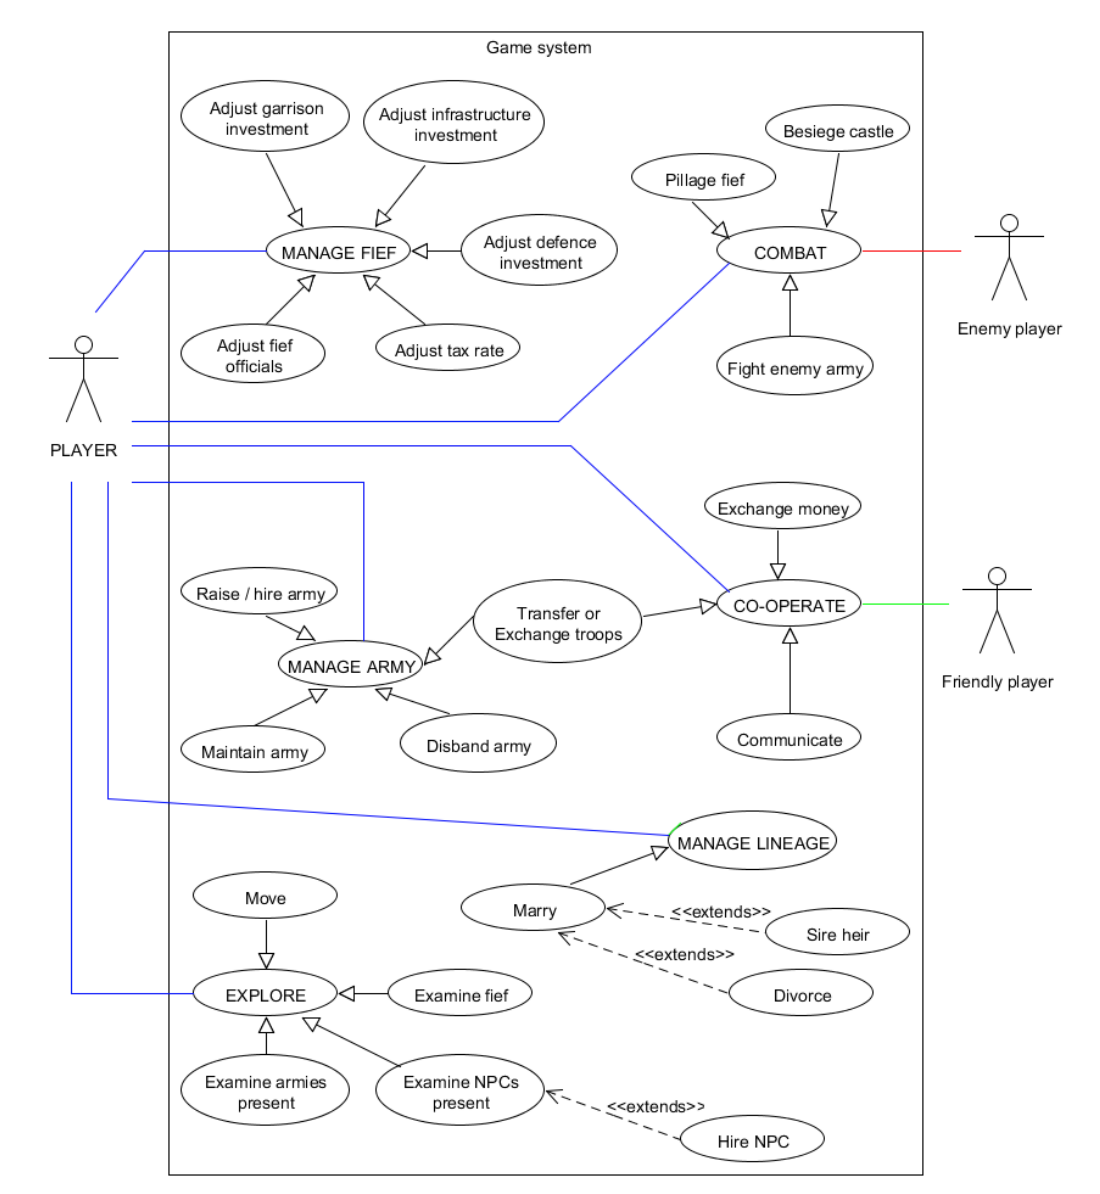
\includegraphics[width=\textwidth]{gameUML}
\end{document}
